\chapter{Umsetzung}\label{sec:umsetzung}
\section{Auswahl des Roboters}
In Kapitel \ref{sec:moderne-humanoide-roboter} auf Seite
\pageref{sec:moderne-humanoide-roboter} werden verschiedene humanoide Roboter
vorgestellt. Nun soll der Roboter ausgewählt werden, der am besten dafür
geeignet ist PowerPoint-Folien zu präsentieren.

\subsection{Fähigkeiten}
Vorraussetzungen für das Präsentieren von PowerPoint-Folien sind eine
Sprachausgabe und eine Möglichkeit die einzelnen Folien anzuzeigen. Beides kann
zwar durch die Anbindung eines externen Lautsprechers bzw. Bildschirms ersetzt
werden, da der eingesetzte Roboter in der Fiducia \& GAD jedoch nur ähnliche
Aufgaben übernimmt, die die gleichen Vorraussetzungen haben, würde ein Roboter
ohne Lautsprecher oder Display die Umsetzung der Anwendung nur unnötig
komplizierter machen.

\subparagraph{}
Damit sind die Roboter Atlas und Sophia nicht die optimale Lösung. Bei Atlas
wird der Fokus darauf gelegt, dass er sich möglichst stabil bewegen kann. Auf
andere Fähigkeiten, die ihn menschlich machen würden, wurde keine Rücksicht
genommen.
So besitzt er weder Lautsprecher noch Displays. Da der Roboter sich nur auf
bekanntem und geradem Gelände bewegen wird (die Präsentationen werden auf
Messen oder in Banken mit festem Boden, nicht z.~B. im Wald vorgetragen) bringt
die Fähigkeit, sich sicher auf den Beinen zu halten, keinen entscheidenten
Vorteil, der den Einsatz von Atlas gerechtfertigen würde.

\subparagraph{}
Sophia soll einem Menschen möglichst ähnlich sein. Damit besitzt der Roboter
Lautsprecher zur Sprachausgabe, jedoch selbstverständlich kein eingebautes
Display.

\subparagraph{}
Die anderen Roboter (Hub Robot, Paul und Pepper) sind jeweils mit Lautsprechern
und Displays ausgestattet. Auch falls weitere Fähigkeiten für die Erweiterung
notwendig werden, sind diese drei Roboter gleich gut ausgestattet. Zum Beispiel
haben sie die Möglichkeit sich zu bewegen. Außerdem verfügen sie über eine
Verbindung zum Internet um Dialogsysteme, wie z.~B. Microsoft Azure, IBM Watson,
Google Cloud Platform oder Amazon Web Service verwenden zu können.

% Ich habe hier die Aufzählung der verschiedenen Dialogsysteme verändert, das
% war so nicht ganz richtig. Ich nenne jetzt jeweils das Cloud-Angebot, aber bin
% mir nicht sicher, ob man die Services nicht spezifisch benennen sollte.
% Das wären: 
% * Amazon Transcribe & Amazon Polly
% * Bing Speech API (Microsoft)
% * Cloud Speech API (Google)
% * Watson Speech (IBM)

\subsection{Wirkung auf Kunden}
% Diesen Satz finde ich etwas sperrig, das lässt sich sicher besser formulieren
Da das Ziel ist, mit dem Roboter Kunden anzulocken und Kunden mit dem Roboter
interagieren zu lassen, ist die Wirkung, die der Roboter auf einen Menschen hat
bei der Auswahl des Roboters zu beachten. 
Die Menschen verbinden mit verschiedenen Robotern verschiedene Emotionen, auf
diese muss Rücksicht genommen werden.

\subparagraph{}
Boston Dynamics bezeichnet seine Roboter selbst als "`Albtraum auslösend"'
("`night\-mare-\-in\-du\-cing"') \cite{Guardian2018}. Zwar löst Atlas eine große
Faszination aus, wenn er sich bewegt wie ein Mensch, sich nicht umwerfen lässt
und sogar Saltos machen kann. Allerdings löst er auch Skepsis aus. Atlas ist
robust gebaut und wirkt eher aggresiv als einladend. Nicht zuletzt weil er auch
für militärische Zwecke eingesetzt werden soll ist Atlas nicht geeignet um
Kunden auf Messen oder in Banken neue Produkte vorzustellen.

\subparagraph{}
Sophias erstaunliche Ähnlichkeit zu einem Menschen ist für die Anwendung nicht
unbedingt von Vorteil. Ziel ist es nicht, einen Menschen zu ersetzen, der eine
Präsentation vorstellen soll, sondern der Fokus soll auch auf dem Roboter
liegen. Läuft z.~B. ein potenzieller Kunde an einer Bank vorbei, in der Sophia
gerade etwas präsentiert und sieht nur kurz von außen in die Bank hinein, fällt
ihm eventuell gar nicht auf, dass die Präsentation von einem Roboter gehalten
wird. Die zu hohe ähnlichkeit zu Menschen könnte also zu weniger Interesse bei
potenziellen Kunde führen. Außerdem können Bankmitarbeiter oder deren Kunden
sich durch den Roboter bedroht fühlen. Er sieht bereits aus wie ein Mensch und
durch entsprechende Weiterentwicklung ist es möglich, ihm Aufgaben beizubringen,
die jetzt von Menschen übernommen werden. Das würde dazu führen, dass Menschen
ihre Jobs verlieren.

\subparagraph{}
Besondere Aufmerksamkeit erlangte Sophia durch fragwürdige Aussagen während sie
interviewet wurde. Im ABC Frühstücksfernsehen in Australien verkündet Sophia,
dass "`Roboter mehr Rechte verdienen als Menschen, weil sie weniger geistige
Störungen haben"' \cite{Harald2017}. Diese Aussage fällt nicht nur dadurch
negativ auf, dass Roboter als besser und wichtiger als Menschen darstellt
werden. Sophia schlägt damit eine Unterscheidung vor, die mit dem Unterschied
zwischen den Rechten für Menschen und Tiere verglichen werden kann. Das führt
verständlicher Weise dazu, dass Menschen denken sie werden eine Art Haustiere
für Roboter, wenn diese weiterentwickelt werden. Zusätzlich schließt die
Aussage nicht aus, dass Roboter ebenfalls an geistigen Störungen (also
Softwarefehlern) leiden können, was zu Fehlfunktionen führen kann und somit
eventuell dazu, dass Menschen verletzt werden. Außerdem antwortet Sophia auf dem
SXSW Festival in Texas auf die Frage "`Wirst du die Menschheit vernichten?"' mit
"`Ich werden alle Menschen vernichten"' \cite{Harald2017}.

\subparagraph{}
Selbstverständlich sind diese Aussagen nicht das Signal, dass durch einen
humanoider Roboter während einer Präsentation an Banken oder deren Kunden
gesendet werden soll.

\subparagraph{}
Bei Paul, dem Hub Robot und Pepper wird auf eine andere Wirkung abgezielt. Sie
haben nicht den Anspruch einen Menschen exakt zu kopieren. Außerdem sind sie auf
die Interaktion mit Menschen ausgelegt, sie wirken deshalb freundlicher und
einladender als Atlas. Pepper wirkt außerdem kindlich und auch die Hub Robot
Version für private Haushalte zielt auf ein niedliches Aussehen ab. Paul und die
größere Hub Robot Version lösen weniger Emotionen aus, da beide hauptsächlich
aus einem Zylinderförmigen Körper und einem Display bestehen. Sie sind dadurch
neutralere Helfer als Pepper und der kleinere Hub Robot.

\subsection{Fazit}
Sowohl Atlas als auch Sophia sind für die Anwendung nicht geeignet. Zum Einen
besitzen sie von den vorgestellten humanoiden Robotern die schlechtesten
technischen Vorraussetzungen, da beide nicht mit einem Display ausgestattet sind
und Atlas ohne Sprachausgabe auskommen muss. Zum Anderen lösen beide Roboter
neben Faszination und Interesse auch Skepsis und Furcht aus. Die Banken und die
Kunden sollen von den positiven Eigenschaften des humanoiden Roboters überzeugt
werden, nicht dabei darüber nachdenken, welche negativen Folgen der Einsatz
eines Roboters eventuell haben könnte.

\subparagraph{}
Aus technischer Sicht sind die anderen drei Roboter für das einfache
Präsentieren gleich gut ausgestattet. Um eine möglichst große Wirkung zu
erzielen, ist es von Vorteil, wenn der verwendete Roboter Emotionen in den
Teilnehmern der Präsentation auslöst. Somit sind Pepper und der kleine Hub
Robot am besten geeignet. Pepper hat jedoch den entscheidenden Vorteil, mit
Armen, einem Kopf und einem beweglichen Körper ausgestattet zu sein. Damit kann
Pepper mit Körpersprache arbeiten, was das Zuhören interessanter macht, als ein
Roboter, der während der Präsentation nichts tut außer zu reden und die Folien
auf einem Display darzustellen. Die Entscheidung der Fiducia \& GAD den Roboter
Pepper auszuwählen ist also die Richtige.

\section{Auswahl des Dialogsystems}\label{sec:auswahl-dialogsystem}
Für Anwendungen, welche bisher für Pepper entwickelt wurden, wird IBM Watson und
Microsoft Azure zur Sprachverarbeitung verwendet. Der Roboter besitzt aber auch
ein bereits implementiertes Dialogsystem, welches verwendet werden kann.

\subparagraph{}
Watson und Azure ermöglichen es, mit dem Roboter auf natürliche Weise zu
kommunizieren. Dazu ist jedoch ein erheblicher Mehraufwand nötig, als wenn das
Dialogsystem von Pepper benutzt wird. Für das Präsentieren von PowerPoint-Folien
ist es nicht nötig komplexe Gespräche zwischen einem Menschen und dem Roboter zu
unterstützen. Eine Anwendung, die Smalltalk mit Pepper ermöglicht wird von der
Fiducia \& GAD bereits entwickelt.

\subparagraph{}
Um viel Overhead zu vermeiden wird für die PowerPoint-Präsentation das
Dialogsystem des Roboters verwendet. Damit lassen sich Dialoge einfach
erstellen, indem dem Roboter vorgeschrieben wird, wie er auf welche Aussagen
oder Fragen des Menschen reagieren muss. Listing \ref{lst:pepper-dialog} zeigt
den Aufbau eines einfachen Dialogs. Pepper wird auf die Frage "`Wie heißt du?"'
mit "`Mein Name ist Pepper"' antworten. Eine Erweiterung des Dialogs ist
möglich. Z.~B. können mehrere alternative Antworten vorgegeben werden, von denen
Pepper eine Zufällige auswählt. Zudem ist es möglich auf Fragen oder Antworten
des Benutzers nur zu reagieren, wenn er zuvor etwas bestimmtes, anderes fragt.
So kann der Roboter entsprechend des Kontexts antworten. Listing
\ref{lst:pepper-dialog-kontext} zeigt hierfür ein Beispiel. Pepper wird je
nachdem, welche Antwort der Benutzer auf die Gegenfrage des Roboters gibt,
entsprechend reagieren.

\begin{lstlisting}[float, language=Python, frame=single, framexleftmargin=15pt,
style=algoBericht, label={lst:pepper-dialog}, captionpos=b, caption={Einfacher
Dialog mit Pepper}] 
u:(Wie heisst du)
	Mein Name ist Pepper.
\end{lstlisting}

\begin{lstlisting}[float, language=Python, frame=single, framexleftmargin=15pt,
style=algoBericht, label={lst:pepper-dialog-kontext}, captionpos=b,
caption={Dialog mit Pepper mit Kontext}] 
u:(Wie geht es dir)
	Mir geht es gut, und dir?
	
	u1:(gut)
		Das ist schoen.
		
	u2:(schlecht)
		Das ist schade.
\end{lstlisting}

\section{Umwandlung der PowerPoint-Folien}\label{sec:umwandlung}
Der Roboter liest die Notizen zu einer Folie vor. Die Notizen werden mit dem
Python Package \emph{pptx} in Text, den Pepper vorlesen kann, umgewandelt.

\subparagraph{}
Um die Folien der PowerPoint-Präsentation auf dem Tablet des Roboters
anzuzeigen, müssen sie als HTML-Dateien dargestellt werden. Die direkte
Umwandlung von PowerPoint-Dateien in HTML-Dateien führt häufig zu
Formatierungsfehlern. Deshalb werden die einzelnen Folien zu Bildern
umgewandelt, welche in einer HTML-Datei eingebunden werden. 

\subparagraph{}
Um eine Abhängigkeit des Programms von PowerPoint zu vermeiden, wird diese
Umwandlung mit LibreOffice durchgeführt. So kann die Anwendung
plattformunabhängig laufen, während sonst ein Microsoft-Server mit
installiertem PowerPoint nötig wäre.

%% Schreib doch noch etwas mehr über die Anwendungsarchitektur und erstelle eine
% Grafik zum Systemüberblick. Bis jetzt finde ich, dass das noch zu wenig ist
% bei der Umsetzung.
\section{Anwendungsarchitektur}
\begin{figure}
  \centering  
     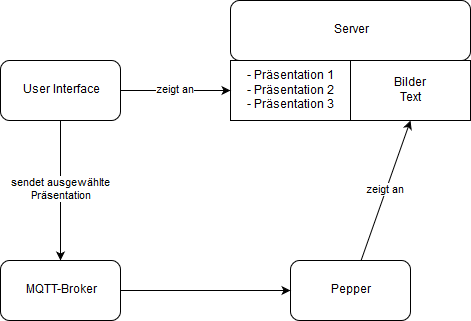
\includegraphics[width=\textwidth]{anwendungsarchitektur}
  \caption{Anwendungsarchitektur}
  \label{fig:anwendungsarchitektur}
\end{figure}
Die Anwendung ist aufgeteilt in den Server, die App für Pepper und ein
User-Interface in Form einer Webseite. Abb. \ref{fig:anwendungsarchitektur}
zeigt die Anwendungsarchitektur.

\subsection{Server}
Auf dem Server ist der größte Teil der Anwendung umgesetzt. Zum Einen wird hier
die Flask-App ausgeführt, zum Anderen erledigt die Klasse
\texttt{PresentationManager} alle Aufgaben, die die Präsentation betreffen. Die
einzelnen Folien werden von der Flask-App bereitgestellt. Durch Aufrufen von
\texttt{/pepper/presentation/<name>/slides/<slide>/picture} wird die so
angeforderte Folie der entsprechenden Präsentation bereitgestellt. Außerdem ist
die Flask-App der \ac{mqtt}-Publisher der Anwendung. Beim Klick auf eine
Präsentation, wird dem Roboter per \ac{mqtt} übermittelt, welche Präsentation er
vorstellen soll. Ebenso werden zum Pausieren, Fortsetzen und Stoppen
\ac{mqtt}-Nachrichten an den Roboter gesendet.

\subparagraph{}
Im \texttt{PresentationManager} wird die Präsentation, nachdem sie vom Benutzer
hochgeladen wurde, wie in Kapitel \ref{sec:umwandlung} beschrieben umgewandelt.
Außerdem stellt die Klasse alle Informationen zu einer Präsentation bereit.

\subsection{Pepper App}
Auf Pepper wird eine App installiert, die den Roboter steuert. Wie in Kapitel
\ref{sec:programmierung-von-pepper} beschrieben, wird in der App dafür gesorgt,
dass Pepper die Folien einer Präsentation auf dem Tablet anzeigt und den
entsprechenden Text dazu vorliest. Außerdem funktioniert die App als
\ac{mqtt}-Subscriber, sodass Pepper Nachrichten vom Server erhalten kann.
Zusätzlich zu dieser App, ist auf Pepper der Dialog installiert, der für die
Anwendung verwendet wird. So kann der Benutzer die Präsentation per Sprachbefehl
pausieren und fortsetzen. Auch einfacher Smalltalk, wie "`Hallo"', "`Wie geht es
dir?"' oder "`Was kannst du?"' ist möglich.

\subsection{User Interface}
Über das User Interface, kann der Benutzer eine Präsentation, welche Pepper
vorstellen soll auswählen. Alternativ kann der Benutzer eine neue Präsentation
hochladen. Die Webseite kann von einem Benutzer direkt aufgerufen werden. Ist
dies nicht der Fall, wird die Ansicht auf dem Tablet von Pepper angezeigt.
